%%
%% This is file `sample-acmtog.tex',
%% generated with the docstrip utility.
%%
%% The original source files were:
%%
%% samples.dtx  (with options: `all,journal,bibtex,acmtog')
%% 
%% IMPORTANT NOTICE:
%% 
%% For the copyright see the source file.
%% 
%% Any modified versions of this file must be renamed
%% with new filenames distinct from sample-acmtog.tex.
%% 
%% For distribution of the original source see the terms
%% for copying and modification in the file samples.dtx.
%% 
%% This generated file may be distributed as long as the
%% original source files, as listed above, are part of the
%% same distribution. (The sources need not necessarily be
%% in the same archive or directory.)
%%
%%
%% Commands for TeXCount
%TC:macro \cite [option:text,text]
%TC:macro \citep [option:text,text]
%TC:macro \citet [option:text,text]
%TC:envir table 0 1
%TC:envir table* 0 1
%TC:envir tabular [ignore] word
%TC:envir displaymath 0 word
%TC:envir math 0 word
%TC:envir comment 0 0
%%
%%
%% The first command in your LaTeX source must be the \documentclass
%% command.
%%
%% For submission and review of your manuscript please change the
%% command to \documentclass[manuscript, screen, review]{acmart}.
%%
%% When submitting camera ready or to TAPS, please change the command
%% to \documentclass[sigconf]{acmart} or whichever template is required
%% for your publication.
%%
%%

\documentclass[acmtog]{acmart}
% \usepackage{graphicx}

%%
%% \BibTeX command to typeset BibTeX logo in the docs
\AtBeginDocument{%
  \providecommand\BibTeX{{%
    Bib\TeX}}}

%%
%% Submission ID.
%% Use this when submitting an article to a sponsored event. You'll
%% receive a unique submission ID from the organizers
%% of the event, and this ID should be used as the parameter to this command.
%%\acmSubmissionID{123-A56-BU3}

%%
%% For managing citations, it is recommended to use bibliography
%% files in BibTeX format.
%%
%% You can then either use BibTeX with the ACM-Reference-Format style,
%% or BibLaTeX with the acmnumeric or acmauthoryear sytles, that include
%% support for advanced citation of software artefact from the
%% biblatex-software package, also separately available on CTAN.
%%
%% Look at the sample-*-biblatex.tex files for templates showcasing
%% the biblatex styles.
%%

%%
%% The majority of ACM publications use numbered citations and
%% references.  The command \citestyle{authoryear} switches to the
%% "author year" style.
%%
%% If you are preparing content for an event
%% sponsored by ACM SIGGRAPH, you must use the "author year" style of
%% citations and references.
\citestyle{acmauthoryear}


%%
%% end of the preamble, start of the body of the document source.
\begin{document}

%%
%% The "title" command has an optional parameter,
%% allowing the author to define a "short title" to be used in page headers.
\title{Propagación de Información en una red Social}

%%
%% The "author" command and its associated commands are used to define
%% the authors and their affiliations.
%% Of note is the shared affiliation of the first two authors, and the
%% "authornote" and "authornotemark" commands
%% used to denote shared contribution to the research.
\author{Alex Sánchez Saez}
\affiliation{%
  \institution{Universidad de la Habana}
  \state{La Habana}
  \country{Cuba}
}
\author{Carlos Manuel González}
\affiliation{%
  \institution{Universidad de la Habana}
  \state{La Habana}
  \country{Cuba}
}
\author{Jorge Alberto Aspiolea}
\affiliation{%
  \institution{Universidad de la Habana}
  \state{La Habana}
  \country{Cuba}
}



%%
%% By default, the full list of authors will be used in the page
%% headers. Often, this list is too long, and will overlap
%% other information printed in the page headers. This command allows
%% the author to define a more concise list
%% of authors' names for this purpose.
\renewcommand{\shortauthors}{Alex,Carlos,Jorge}

%%
%% The abstract is a short summary of the work to be presented in the
%% article.
\begin{abstract}
 Este es el resumen Técnico de nuestro proyecto de IA-Simulación para el Curso 2024 , En este proyecto nos propusimos responder a las siguientes interrogantes; ¿Como se difunde la Información en una Red Social? y ¿Sabiendo esto podremos crear una Publicación que se adecúe a nuestras necesidades y que tenga el Mayor crecimiento Posible? . Para responder a esto Creamos una herramienta basándonos en los conocimientos adquiridos en las asignaturas de IA y Simulación y datos recopilados a través de la Investigación y revisión de la bibliografía disponible
\end{abstract}


\keywords{Simulación, Inteligencia Artificial, Red Social}

%%
%% This command processes the author and affiliation and title
%% information and builds the first part of the formatted document.
\maketitle

\section{Introducción}
Este es el Resumen Técnico de nuestro proyecto de IA-Simulación para el Curso 2024. En este proyecto nos propusimos responder a las siguientes interrogantes: ¿Cómo se difunde la Información en una Red Social? y ¿Sabiendo esto, podremos crear una Publicación que se adecúe a nuestras necesidades y que tenga el Mayor Crecimiento Posible? Para abordar estas cuestiones, creamos una herramienta basada en una interfaz en lenguaje natural para interactuar con el usuario, además de una simulación multiagente con arquitectura BDI. Este enfoque nos permitió aprovechar los conocimientos adquiridos en las asignaturas de IA y Simulación, así como los datos recopilados a través de la investigación y revisión de la bibliografía disponible.

\section{Acerca de la Difusión de la Información en Redes Sociales}
Como Parte de nuestra investigación para la creación de este proyecto , nos dimos a la tarea de encontrar y comprender el estado del arte en la representación y análisis computacional de los sitemas sociales complejos como las Redes sociales. Estudiamos El panorama Histórico de la Modelación de este tipo de problemas y Su relación con el Modelo SIR para la propagación de epidemias \url{https://theconversation.com/covid-19-y-difusion-de-innovaciones-parecidos-razonables-157385}. Dimos con el Modelo de Difusión de opiniones de Rogers el cuál explica la dinámica de las opiniones a una macro escala , sin tener en cuenta los eventos locales \url{https://www.eurekando.org/ciencias-sociales/teoria-de-la-difusion-de-rogers-innovacion-y-difusion/}. Analizamos también algunos Modelos Clásicos utilizados para analizar este tipo de problemas. Los problemas Binarios eran simulaciones multiagente donde los agentes tenian solo dos posibles opiniones respecto a un tema -1 o 1 . La forma en que se difundían estas opiniones era variada en dependencia del autor , algunos ejemplos son : Propagación de opiniones por vecinos cercanos (Modelo de Voter) , Opinión Mayoritaria del grupo al que pertenece el agente (Modelo de Majority Rule) , Propagación por los Vecinos con la misma Opinión (Modelo Szrajd) . Una evolución a estos modelos son los modelos Continuos o Modelos Socio-Físicos en los cuales ya los agentes tienen opiniones no binarias , osea un grado de seguridad respecto a su postura con el tema . Algunas formas de propagación de opiniones en estos modelos son : A través de un confidence level o nivel de confianza , esto significa que cuando dos agentes interactúan varían sus opiniones según su nivel de confianza hacia esta (Deffort y Hegselmann-Krausse). 

\subsection{Nuestro Modelo de Simulación}

Nuestra simulación es un sistema multiagente que usa la arquitectura BDI para modelar el comportamiento de un usuario humano dentro de la red .El medio donde se colocan los agentes es una red donde cada agente tiene un nivel de confianza con el resto de agentes , esto es un valor [-1,1] donde 0 significa que el agente (visto como un nodo ) está completamente desconectado y el resto indica que tan bien o mal le cae el otro agente . Las interacciones posibles que tienen los agentes son : dar like a la publicacion i , dar dislike a la publicacion i , compartir la publicacion i , con el agente j 

\subsection{Representación de los datos}
Nuestro sistema desde el punto de vista de los modelos Socio-Físicos es un modelo multitema tipo CODA (Continous Opinions , Discrete Actions) esto debido a que manejamos las opiniones como un parametro privado de los agentes individuales , y estos solo tienen un rango discreto de acciones a realizar .Representamos las Publicaciones al igual que las opiniones como arreglos de numeros , en el caso de las publicaciones numeros entre 0 y 1 que representan que tan relevante es el tema en la publicacion ; y en el caso de las opinione de los agentes serían numeros entre -1 y 1 que representan que tan de acuerdo esta el agente con el tema en cuestión 

\section{Agentes}
Cada agente tiene 7 parámetros que definene su comportamiento , estos son sus valores de afinidad que es su opinion respecto a los temas presentes en la red se representa con un array de numero con valores que estan en [-1,1].Trust Afinity que es el valor de confianza que tiene respecto al resto de agentes de la red , se representa como un diccionario de pares (id del agente,valor de confianza) , donde el valor de confianza es un numero [-1,1].Like, Dislike y Share tresholds , son los umbrales para determinar si el agente realizara alguna de esas acciones.Others impact, Extroversion y Group Conformity , estos representan la componente social del agente con estos parametros se definira como asimila la información que obtiene del resto de los agentes. Reaction treshhold y Curiosity , representan la curiosidad y la pereza de los agentes , definen cuando el agente reacciona o no a una publicación que llega o a una publicación de alguien que no conoce. Friends definition , afinity treshold y relevance treshold le ayudan al agente a tomar decisiones , con Friends definition determina que usuarios consideras miembro de su grupo o subred y con los otros dos define la forma en que valora un post (en base a su afinidad personal o la relevancia colectiva)

\section{Acciones que ejecutan los Agentes y Cómo lo hacen}
En cada Step de la simulación los agentes tendran en sus intentions las acciones que quieren realizar y por cada una de ellas , las ganas que tienen de realizarlas, se toman entonces las N primeras acciones a realizar por el agente , donde N es un número aleatorio y se mandan a realizar , las acciones posibles a realizar por parte de los agentes son : Dar like a una publicación , dar dislike a una publicación , compartir la publicación i con el agente j. Al reaccionar a una publicación los agentes calculan cuán alineadas están las características de dicha publicación con sus gustos, y la relevancia que tiene esa publicación para su grupo , esto lo hace revisando cuantos de los usuarios que pertenecen a su grupo (con los que tenga mas confianza que su Friend definition) y viendo cuáles de estos han dado like a la publicación , tomando esto en cuenta calcula el nivel de gusto que tiene hacia el post en cuestión , luego verifica cuántas de las publicaciones que recuerda son muy similares a esta; Para simular la memoria de un agente guardamos solo las publicaciones que más les hayan impactado , ya sea positiva o negativamente ya que similar a esto funciona la memoria humana , aunque tomando muchas simplificaciones; Si la publicación es algo que el agente ha visto mucho , se penaliza el nivel de gusto , o nivel de relevancia de la publicación al agente .Si la publicación le fue enviada por otro usuario actualiza su relación con él , para esto se tiene en cuenta cuánto le gustó la publicación enviada y las experiencias pasadas con el agente (tanto positiva como negativas , ambos tiposs de interacciones pasadas afectan de manera diferente).De igual manera en haciendo uso de la componente de extroversión del agente se toma la decición de compartir la publicación con el resto de agentes de la red. Teniendo en cuenta el impacto que tienen los demás al agente y cuál es su nivel de conformidad grupal , se ajustan sus afinidades a la publicación vista. Una vez pasado todo este proceso se decide si dar like o dislike a la publicación .Todo esto solo puede pasar si el agente tiene ganas de reaccionar a la publicación , esto se calcula teniendo el cuenta la curiosidad y la pereza del agente

\section{Generación de los datos iniciales para la simulación}
Todos los datos que se utilizan se generan de manera aleatoria utilizando distribuciones normales que se ajustan mas al comportamiento de los parámetros en una población .Variando la media y la desviación estándar de dichas distribuciones ajustamos la generación de los parámetros a lo que pide el usuario y al análisis que se hace después 

\section{Análisis de resultados}
Una vez se han hecho las simulaciones Tomamos varios datos , en primer lugar vemos la relación de las métricas por publicación (likes,dislikes y veces compartida) para tener una idea de que publicaciones han triunfado más en la red .Según cuáles sean las carácterísticas que se quieran analizar se toman los posts en donde estas características tengan grado de pertenencia mayor a 0.6 y calculamos sus índices de crecimiento (promedio de sus likes , dislikes y veces compartido) para poder analizar el crecimiento de estos temas en la red. También analizamos lass opiniones de los usuarios respecto a los temas dispuestos para analizar ; esto nos sirve para determinar que post tiene mejor rendimiento en la red según las necesidades del usuario

\section{Criterios de Parada}

Cada Simulación Individual se detiene cuando los usuarios dejan de interactuar con los posts de la red .Los Datos Obtenidos por la simulación van a depender de como se generan las variables que se usan , por lo que es poco probable que converjan de alguna manera , es por esto que como criterio de parada se le deja a eleccion del usuario que cantidad de simulaciones se pueden correr en dependencia de su hardware y recursoss

\section{Procesamiento del Lenguage Natural (NLP)}

El flujo de simulación empieza por pedirle al usuario algunos datos relacionados al estado de la red social que él desea simular y que objetivos tiene con la simulación.
Dichos datos están conformados la cantidad de personas en la red social, una \textbf{descripción} de la red social a simular, de donde se extraerán los tos temas más 
relevantes que se mencionan comúnmente y los objetivos que tiene  el usuario con la simulación.
\\
Para esto se usará el procesamiento del lenguage natural, en donde el usuario introducirá un texto mencionando cuantos usuarios tendrá la red, una breve descripción de los
temas que se tratan en la misma y una explicación de sus objetivos con la simulación.
\\
Luego de tener el texto usaremos uno \textbf{Large Language Model (LLM)} para extraer la información necesaria del input del usuario.
Para realizar una extracción más detallada, se realizaron 3 consultas al LLM: 

\begin{itemize}
    \item Una primera consulta en donde simplemente el LLM extrae la cantidad de personas que habrán en la red social.
    \item Una segunda consulta en donde el LLM analiza el texto y extrae los temas más relevantes que se ven en la red social y que le asigne a cada tema un número indicando el porcentaje de personas que les intereca comúnmente ese tema.
    \item Y una tercera consulta en donde el LLM analiza el texto y extrae, basado en los objetivos que expresa el usuario, tres números que representan qué tan importante son los \textbf{likes}, \textbf{dislikes} y \textbf{shares} en la simulación para lograr los objetivos del usuario.
\end{itemize}

Para obtener correctamente los datos del texto del usuario se exigió que el \textit{prompt} tenga al menos $100$ palabras para que sea lo suficientemente expresivo, además de usar algunas técnicas de \textbf{Prompt Engineering} como darle un rol al modelo, especificarle un formato específico para
la salida y realizar consultas con tareas simples y directas.

\subsection{Importancia de los temas en la red}

Una vez se extraen los datos usando el LLM, tocaría llevar los temas proporcionados por el modelo al conjunto de temas que tenemos preestablecidos. Para esto vamos usar la representación en \textbf{embeddings} de cada tema (incluido los proporcionados lor el LLM),
así podemos hacer una una comparación semántica de cómo de relacionados están dos temas usando la \textit{distancia coseno}.
\\
Supongamos que tenemos $n$ temas preestablecidos en nuestra red social, nuestro objetivo es construir un vector $v$ de $n$ elementos donde $v_i \in [0,1]$ representa que tan relevante es el tema $i$ en la red social. Sea $m$ la cantidad de temas devueltos por el LLM y $p_i$ la importancia dada a cada una en la red.
Si tenemos los embeddings de cada grupo de temas(sean $a$ y $b$ respectivamente), entonces la para calcular la relevancia $v_i$ del tema $i$ en la red social basado en los $m$ temas principales devueltos por el LLM podemos calcularlo como:

$$
v_i = \frac{\sum_{j=1}^{m} p_j sim(a_i, b_j)}{n},  \forall 1 \leq i \leq n   
$$

donde $sim(a_i, b_j)$ es la similitud entre los temas $i$ y $j$ usando los embeddings de cada uno.
\\
Esta suma ponderada de la similitud de los temas devuelto por el LLM multiplicados por la importancia que tiene cada una en la red social, nos da una medida aproximada de la relevancia del tema $i$ en la red social.


\subsection{Representación del conocimiento}
Con los embeddings calculados , podemos crear una base de conocimiento sobre los temas de la red , que nos ayude a razonar sobre la relación que existe entre lso diferentes temas que existen en esta . Para esto calculamos una matriz de correlación que nos dice que tan relacionado está un tema con el resto. Esto lo utilizamos para ajustar los parámetros en la generación de los posts de manera que sea coherente y se ajuste a la petición del usuario de nuestro sistema , digamos que el usuario quiera que la mayoria de sus posts hablen mucho de tecnología , eso implicaría que tecnología debe tener una media más alta que el resto de temas , a su vez , temas que guarden cierta relación con la tecnología deben tener medias semejantes y otros temas muy bajas , porque no tendrán relación con lo que se maneja en la red , esto nos sirve para que la forma de las publicaciones al ser generadas tengan mas coherencia y sean más realistas


\section{Optimización}

Una vez la simulación arroge las estadísticas antes mencionadas, ahora tenemos la interrogante de encontrar \textit{¿qué combinación de temas y en qué cantidad proporciona un mejor alcance en la red?}.
Esta interrogante tiene dos pasos importantes; primero, ¿cómo calificas que una publición proporciona mayor alcance?¿bajo que criterio es interesante realizar una búsqueda de la mejor solución? y
en segundo lugar tenemos el problema de \textit{¿Cómo vamos a encontrar dicha solución óptima?}

\subsection{Criterios de optimalidad}

Para responder la primera pregunta, podemos ver que cada post en la red social se mide por tres estadísticas principales: \textit{cantidad de likes, cantidad de dislikes y veces compartida}, además que
la simulación nos proporciona esas mismas estadísticas enfocándonos esta vez en el tipo de tema, por tanto tendríamos un índice de que tanto gusta cada tema entre los usuarios (cantidad de likes promedio),
o cual es el tema que menos gustó (cantidad de dislikes promedio), o incluso cuáles son los temas que más se difundieron, ya sea por gustos o disgustos, en la red(cantidad de veces compartida). Entonces depende
de los intereses del tengamos podemos decidir que importancia darle a cada una de esas tres estadísticas.


\subsection{Encontrar la mejor solución}

Para la segunda pregunda \textit{¿cómo encontrar la mejor solución?}, debemos fijarnos que la solución consiste en un vector $x$ de tamaño $n$, donde cada componente del vector es un número $x_i \in [0,1]$ que
indica que el tema $i$ debe tener una relevancia $x_i$ en el post para que tenga el mayor alcance.
\\
Para saber si una solución es mejor que otra debemos tener una forma de cuantificar dicha mejora y así poder hacer la comparación. Para esto definimos una función $f: D \rightarrow \mathbb{R}$, donde $D$ es
el dominio de todas las soluciones posibles del problema, o sea, todas las formas posibles en las que se puede construir un post, y $f(x) \in \mathbb{R}$ un número que indica que tan buena es la solución. 
Podemos ver que $D$ es de tamaño infinito, ya que una solución consiste en una distribución de $n$ números entre $0$ y $1$, y como este conjunto es no enumerable entonces hay infinitas combinaciones de $n$ números
que pertenezcan al rango $[0, 1]$.
\\
Por ende, una buena forma de enfrentar el problema es usando metaheurísticas para encontrar a la función objetivo $f$ un óptimo que se aproxime a la solución real. Como metaheurística usamos \textbf{Particles Swarm Optimization (PSO)}, que nos permite tener un enfoque multiagente para explorar el espacio de las soluciones y una implementación sencilla.

\subsection{Función de optimización}

En la simulación existen $n$ características que describen los diferentes temas de los que puede tratar un post. Cada post en la red social tiene un vector $v$ de $n$ dimensiones con valores $v_i \in [0, 1]$ que indica que tan relevante es el tema $i$ en el post.
También, de la simulación se extrae para cada característica, tres indicadores importantes(Likes, dislikes y veces compartida). Por tanto, podemos crear una matrix $C{n,3}$ donde $C_{i,j}$ indica que porcentaje de la red tuvo la reacción $j$ en posts donde el tema $i$ es relevante.
\\
El objectivo es entonces encontrar el vector $v$ tal que tenga la mejor combinación de relevancias por cada característica y nos dé el mayor crecimiento en la red. Como el impacto de una post de un tema $i$ se mide por los 3 índices expuestos anteriormente (`likes`, `dislikes`, `shares`), 
entonces necesitamos un valor que indique cuan relevante es este índice para un post. Sea $\alpha, \beta, \lambda \in [-1, 1]$ los respectivos indices de relevancia, en donde $-1$ afecta muy negativamente al post y $1$ afecta muy positivamente al post.
Por otro lado para medir el impacto de una publicación en la red esta se podría calcular como:

$$
I(v) = \alpha g_1(v) + \beta g_2(v) + \lambda g_3(v)
$$

donde $g_1(v), g_1(v)$ y $g_1(v)$ indican cuanto afectan los indices de crecimiento respectivamente entre todos los temas.

La forma de calcular las 3 funciones son la misma, solo que se separan en funciones diferentes para mejor comprensión. Para esto hacemos uso de la función exponencial para recompenzar las a los valores mas grandes de $x$. Entonces podemos definir la función $g_1(v)$ que indica cuanto ... como:

$$
g_1(v) = v_1 \alpha e ^ {\sum_{i=1}^{n} C_{i,1}} 
$$

Entonces la función en su totalidad la podemos expresar como:

$$
I(v) = \alpha g_1(v) + \beta g_2(v) + \lambda g_3(v) = v_1 \alpha e ^ {\sum_{i=1}^{n} C_{i,1}} + v_2 \beta e ^ {\sum_{i=1}^{n} C_{i,2}} + v_3 \lambda e ^ {\sum_{i=1}^{n} C_{i,3}}
$$

Si definimos el vector $z = [\alpha, \beta, \lambda]$ entonces la función quedaría:

$$
I(v) = \sum_{j=1}^{3} z_j v_i  e ^ {\sum_{i=1}^{n} C_{i,j}}
$$

Ahora bien, como queremos hallar el vector $x$ tal que maximize el impacto en la red entonces tenemos que optimizar la funcion $I$ para calcular el máximo:

$$
\max I(v) = \max \sum_{j=1}^{3} z_j v_i e ^ {\sum_{i=1}^{n} C_{i,j}}
$$


\section{Algunas ideas que no se llegaron a implementar}
La posibilidad de que los agentes falseen sus opiniones como pasa a menudo en internet fue una de las posibilidades que no implementamos dada su complejidad . Agregar más acciones posibles a los agentes, teníamos la idea de permitir comentarios (positivos y negativos) así como mensajes los cuales podríamos llevar a lenguaje natural usando el LLM, por temas de tiempo y complejidad no llevamos esta idea a cabo. Agregar más control sobre la simulación por parte del usuario, con una buena descripción de la red se podrían extraer más parámetros para la simulación, como serían la extroversión de los agentes de la red, la posibilidad de simular varias redes con distintas distribuciones de agentes, controlar la forma en que se generan las relaciones de los agentes, así como generar grupos de fanáticos o excépticos, como se genera la topología de la red también sería un aspecto interesante a agregar. Respecto al análisis de los datos, se podría agregar un análisis de los grupos sociales que se crean depués de cada simulación para analizar como se agrupan los usuarios de la red

\section{Conclusiones}
Con este trabajo se llegan a conclusiones sobre la forma en que se crean y conectan las opiniones en internet, en un entorno de red social muy simplificado. Podemos llegar a análisis interesantes sobre como se comporta la influencia social para los usuarios de una red a través de la modelación e interacción de usuarios de distintos tipos y cómo se influencian entre ellos. Se puede analizar como las estrategias de marketing se pueden optimizar a través de un conocimiento muy general del público objetivo y el ambiente donde se lanzará la campaña.

\section{Algunos resultados experimentales}

Usando el siguiente prompt como entrada para \textit{Claude}:

\begin{quote}
  \textit{My community in discord has around of 50 people. Here, i share content about programming and software development mainly. Often i share content about artificial intelligence and the people like it so much. Also i make some posts about my career in the software development. Generally, people like AI content much more than personal growth content. I would like to be able to continue creating content in a smarter way to grow my community and reach the greatest number of people possible, and help them in their professional life.}
\end{quote}

Aquí especificamos que la comunidad es de 50 personas y que a menudo se comparte contenido sobre programación, inteligencia artificial y crecimiento personal. También se mencionan los gustos que tiene la comunidad a estos temas para dar información de que tan relevante es cada tema.
Por último se menciona los objetivos que se quisieran alcanzar en esa comunidad, en este caso, hacer crecer la comunidad y poder ayudar a las personas.
\\
Con este \textit{prompt}, el LLM, mediante las tres consulas que se le hacen para procesar los datos pudo concluir que:

\begin{itemize}
  \item La \textbf{cantidad de personas} de la comunidad es $50$.
  \item Temas relevantes: \textbf{Programming} con $0.8$ de relevancia para la comunidad, \textbf{Software Development} con $0.8$, \textbf{Artificial Intelligence} con $0.9$, \textbf{Career in Software Development} con $0.6$, y finalmente \textbf{Personal Growth} con $0.5$.
  \item Cuantificación de sus objetivos: \textbf{likes} un $0.8$, \textbf{dislikes} un $0.3$ y \textbf{shares} un $0.7$.    
\end{itemize}

Analizamos ahora cada uno de los puntos anteriores. 
\\
Para identificar el tamaño dela comunidad no  hubo problemas ya que estaba bastante explícita.
\\
En los temas relevantes nos seleccionó varios pero asignó correctamente los pesos, ya que la comunidad de manera general trata sobre programación, aunque con un gusto un poco más específico por la inteligencia artificial. 
Ahora bien, estos temas para un mismo prompt varian, por tanto para poder llevar estos temas genéricos a temas epecíficos de nuestro conjunto de datos, se usó la comparación entre \textit{embeddings} y quedándonos con los temas que más
se asemejan los extraidos. En este caso se indentificaron los temas: \textbf{Game Development}, \textbf{Artificial Intelligence}, \textbf{Career Development}, \textbf{Personal Finance}.
\\
Después de realizada la simulación y realizada un análisis estadístico se obtubieron los sugientes datos:

% \begin{figure}[h]
%   \centering
%   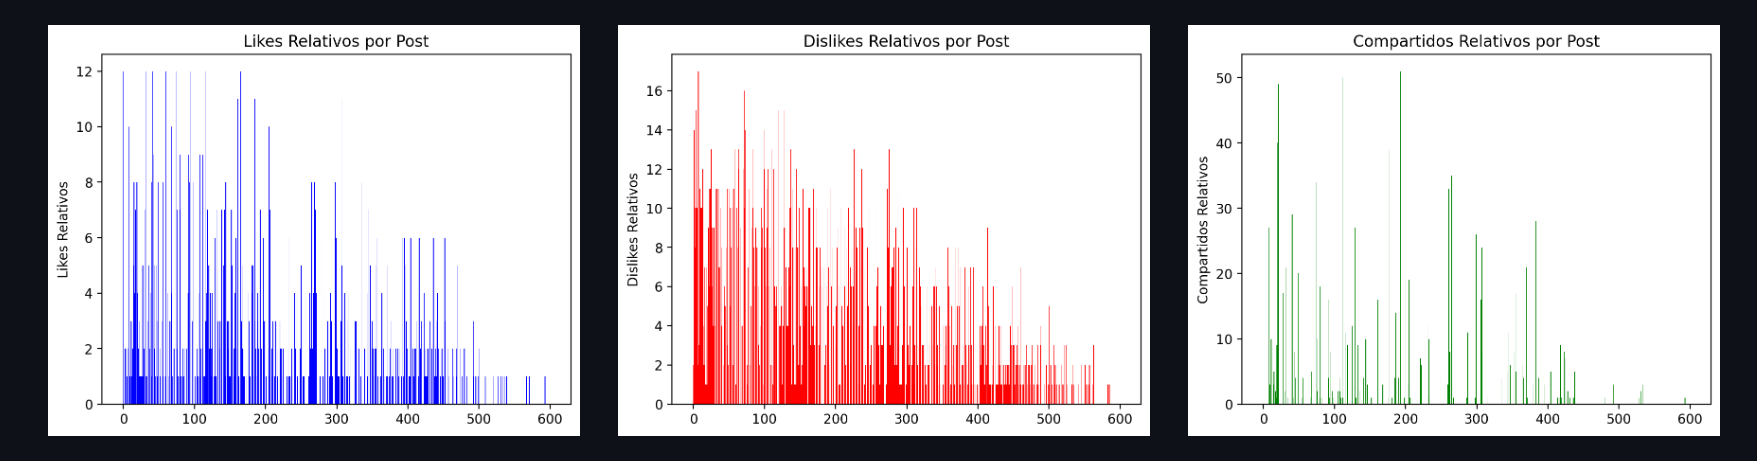
\includegraphics[width=\linewidth]{an_1-lds.png}
%   \Description{Indice de likes, dislikes y veces compartida de los posts}
% \end{figure}

\end{document}
\endinput
